\documentclass[orivec]{llncs}

\usepackage{algorithmic}
\usepackage{pdfsync}
\usepackage{graphicx}
\usepackage{wrapfig}

\newcommand\dually{{\bf D}{\sc U}{\bf AL}{\sc L}{\sc y}}
\newcommand\name{{\sc byADL}}
\newcommand\charmy{{\sc Charmy}}

% partial maps
\newcommand{\pto}{\rightarrowtail}
% domain of a partial map
\newcommand{\pmapincluded}{\subseteq}
% typed graphs: underlying graph
\newcommand{\tgr}[1]{\ensuremath{|{#1}|}}
% typed graphs: underlying morphism
\newcommand{\tmap}[1]{\ensuremath{\tau_{{#1}}}}
% category of T-typed graphs with partial morphisms
\newcommand{\PTyped}[1]{\ensuremath{{#1}\mbox{-}\mathbf{PGraph}}}
% domain of a partial map
\newcommand{\dom}[1]{\ensuremath{\mathit{dom}(#1)}}

\def \mathrule #1#2#3{\begin{array}{l}%
    {\mbox{\scriptsize ({\sc #1})} }%
    \\ \irule{#2}{#3}%
\end{array}}
\newcommand{\irule}[2]{\frac{\textstyle\rule[-1.3ex]{0cm}{3ex}#1}%
{\textstyle\rule[-.5ex]{0cm}{3ex}#2}}

\def \mathaxiom #1#2{\begin{array}{l}%
    {\mbox{\scriptsize ({\sc #1})} }%
    \\ \iaxiom{#2}%
\end{array}}
\newcommand{\iaxiom}[1]{\textstyle\rule[-1.3ex]{0cm}{3ex}#1}

\def \mathruleside #1#2#3#4{\begin{array}{l}%
    {\mbox{\scriptsize ({\sc #1})} }%
    \\\irule{#2}{#3} \;\;\scriptstyle{#4}%
\end{array}}

% *** ALIGNMENT PACKAGES ***
%
\usepackage{array}
\usepackage{mdwmath}
\usepackage{mdwtab}
\usepackage{amsmath}
\usepackage{amssymb}
\usepackage{url}
\usepackage{times}

% Macros for proof-reading
\usepackage[normalem]{ulem} % for \sout
\usepackage{xcolor}
\newcommand{\ra}{$\rightarrow$}
\newcommand{\ugh}[1]{\textcolor{red}{\uwave{#1}}} % please rephrase
\newcommand{\ins}[1]{\textcolor{blue}{\uline{#1}}} % please insert
\newcommand{\del}[1]{\textcolor{red}{\sout{#1}}} % please delete
\newcommand{\chg}[2]{\textcolor{red}{\sout{#1}}{\ra}\textcolor{blue}{\uline{#2}}} % please change

% Put edit comments in a really ugly standout display
\usepackage{ifthen}
\usepackage{amssymb}
\newboolean{showcomments}
\setboolean{showcomments}{true} % toggle to show or hide comments
\ifthenelse{\boolean{showcomments}}
  {\newcommand{\nb}[2]{
    \fcolorbox{gray}{yellow}{\bfseries\sffamily\scriptsize#1}
    {\sf\small$\blacktriangleright$\textit{#2}$\blacktriangleleft$}
   }
   \newcommand{\version}{\emph{\scriptsize$-$working$-$}}
  }
  {\newcommand{\nb}[2]{}
   \newcommand{\version}{}
  }

\newcommand\ivano[1]{\nb{Ivano}{#1}}
\newcommand\henry[1]{\nb{Henry}{#1}}
\newcommand\marco[1]{\nb{Marco}{#1}}



% end Macros for proof-reading


\begin{document}

\title{{Developing an automatic bridge between UML profiles and MOF metamodels}
\thanks{This work is partly supported by the Italian PRIN d-ASAP project.}}

\titlerunning{Developing an automatic bridge between UML profiles and MOF metamodels}

\author{Ivano Malavolta, Henry Muccini, Marco Sebastiani}
\institute{University of L'Aquila, Dipartimento di Informatica\\
\email{\{ivano.malavolta,henry.muccini,marco.sebastiani\}@univaq.it}}

\authorrunning{Malavolta, Muccini, Sebastiani}\maketitle

\begin{abstract}
In Model Driven Engineering, UML profiles and MOF-based Domain Specific Modeling Languages are the most used approaches for specifying and documenting a system in the context of a specific domain.  
The choice of the right approach depends on several aspects, such as tool support, expressivity, complexity of models, company policies. In general, profiled UML models are very much used since they are intuitive for designers and model editors already exist, however they are intrinsically complex for tools manipulating them; conversely, DSML models are more concise and easy to be manipulated, but they require an initial effort in terms of designers training and model editors development. 
%What happens today is that UML is widely used by designers, but the underlying tools suffer from the complexity of the models. 

In this paper we propose an approach that allows to get the best of the two worlds: 
on one side designers describe the system using a familiar UML profile, on the other side the tool manipulates DSML models. Our approach is based on an automatic bridge between UML profiles and MOF metamodels (which are the basic artifact of MOF-based DSMLs). The bridge is transparent to the user since it autonomously operates both on UML profiles 
%(and their associated MOF metamodels) 
and all the involved models. The bridge is realized through model transformation techniques in the Eclipse platform. In this paper we show its application on a case study based on SysML.


%In Model Driven Engineering, the use of UML profiles and Domain Specific Modeling Languages are the most used approaches for specifying and documenting a system. The choice of the right approach depends on several aspects, such as tool support, expressivity, complexity of models, company or organization policies. What happens today is that in many UML-based approaches, models are intrinsically complex and the application of a profile on them exarcebates this situation; this complexity affects also the other artifacts (e.g., model transformations, graphi) associated to the
%
%
 %profiling and the use of a DSML are mutually exclusive. This precludes the possibility to benefit from both techniques while design the system of interest.
%This paper presents an approach for bridging UML profiles and MOF metamodels with a focus on automation. Indeed, the proposed mechanism is fully automatic and operates at both metamodelling and modelling levels. The approach is realized through model transformation techniques in the Eclipse platform.
\end{abstract}

%-------------------------------------------------------------------------
\section{Introduction}\label{sec:intro}

Domain specific applications require notations enabling to capture specificities of the domain, at the right level of abstraction. Domain Specific Languages (DSLs~\cite{FowlerBook}) have been introduced for this purpose, facilitating the specification of domain information. In Model Driven Engineering (MDE), UML profiling~\cite{UML} and Domain Specific Modeling~\cite{DSML} are the most used techniques for defining a DSL.

The \textit{UML profiling} technique consists in extending the UML modeling language with concepts coming from
the domain of interest \cite{UMLprofile}.
A UML profile is the definition of such an extension; the application of a profile to a UML model allows to tailor it with domain-specific information, by specializing existing UML meta classes. Among the most popular UML profiles, we can cite SysML\footnote{Official OMG SysML site: \small{\url{http://www.omgsysml.org}}}
for modeling systems engineering applications, and
MARTE\footnote{Official OMG MARTE site: \small{\url{http://www.omgmarte.org}}} for real-time and embedded applications.
%and
%EAST-ADL\footnote{EAST-ADL specification site: %\small{\url{http://www.atesst.org}}} for automotive %electronic systems.

The \textit{Domain Specific Modeling} technique consists in defining and using languages dedicated to a specific domain.
Those languages are called Domain Specific Modeling Languages (DSMLs) and their concepts are usually formalized  via MOF metamodels~\cite{MOF}.
Each language can have its textual or graphical representation, and tool support can be provided either by generic (meta-modelling tools) or
ad-hoc modeling environments~\cite{DSML}.
Examples of DSML are: AADL to model embedded real-time systems~\cite{aadl}, Backbone for component-based applications~\cite{backbone},
and BPMN for business processes~\cite{BPMN}.

Currently, in many MDE projects both UML profiles and DSMLs are extensively used and each technique has its own strengths and weaknesses,
depending on the needs of the various stakeholders.
The choice of the right approach depends on several aspects, such as tool support, language expressiveness,
models complexity, and company policies~\cite{comparison}.
%In general, profiled UML models are very much used since they are intuitive for designers and model editors already exist, however they are intrinsically complex for model manipulation (e.g., transformation, analysis); conversely, DSML models are more concise and easy to be manipulated, but they require an initial effort in terms of designers training and model editors development.
%A detailed discussion on how the two techniques differ is provided in .
%Determining which is the best technique is not in the scope of this paper
%and there are many cases in which they are used together in order to complement each other \cite{AAA}.
What can be noticed today is that UML profiles became extremely popular, and used as an extensive tool for describing domain specific
applications.
However, while of more immediate use for practitioners (since a profiled model is essentially an annotated UML model that can be
created using existing UML tools), developing a tool to manipulate profiled UML models is a complex activity; this is a consequence
of the inherent complexity of the involved models~\cite{comparison}\cite{france}.
Such a complexity is mainly due to
(i) the intricacy of the UML language, where many strictly related concepts are scattered across its metamodel (the so called "metamuddle"\cite{france})
, and (ii) because the application of a profile imposes additional constraints in the way models are manipulated~\cite{UMLprofile}.
For example, profiles and stereotypes can only be applied in a fixed order, tagged values are accessed through ad-hoc mechanisms, and so on.
It is important to note that the complexity of manipulating profiled UML models is not strictly related to
the system of interest, but relies on the profiling technique itself.
%so we can consider it as an accidental complexity.

Goal of this work is to support those kind of projects in which the system is modelled using UML profiles, and there is a strong need of automatic model manipulation (e.g., to perform some kind of analysis~\cite{UMLprofilesAnalysis}).
This paper proposes a fully \textbf{automatic bridge} between UML profiles and MOF metamodels; such a bridge alleviates the accidental difficulty in manipulating profiled UML models, without forcing designers to abandon UML-based notations.
By using the bridge, on one side designers can describe the system using UML profiles, and on the other side tools operate
on \textit{automatically generated} MOF-based models.
The bridge is totally transparent to designers since it operates at both metamodeling and modeling levels of abstraction.
%that is, designers can continue to develop models using UML profiles, and the bridge manages to transform them to MOF-based models.
At the metamodeling level, the bridge automatically generates a MOF metamodel $MM_x$ representing the concepts of each UML profile.
At the modeling level, it automatically transforms each profiled UML model to a model conforming to $MM_x$, and vice versa.
%This unveils one of the advantages of our approach: designers interact with UML models and the tools manipulate only MOF-based models.
Since designers typically use only a small subset of the UML diagrammatic elements~\cite{france},
it is fundamental to generate a MOF metamodel that contains only such UML elements, while discarding any other information; for this purpose, a \textbf{slicing mechanism} is presented. The proposed bridge is implemented as an Eclipse\footnote{The Eclipse Foundation open source community website: \small{\url{http://www.eclipse.org}}} plugin. The Eclipse platform enables the integration of the bridge
with other technologies available in the Eclipse community. In this paper we show application of the proposed bridge on a case study based on OMG Systems Modeling Language (SysML). It is important to clarify that while this work might not provide some novel theoretical results, it provides a concrete solution to a problem that exists in practice.

The remainder of this paper is organized as follows. In Section~\ref{sec:motivation} we discuss the main motivations for our work.
We describe our automatic bridge in Section~\ref{sec:framework} and the mechanism for slicing the obtained MOF metamodel
in Section~\ref{sec:slicing}. Then, Section~\ref{sec:tool} gives some implementation details, and Section \ref{sec:caseStudy} describes the application of the proposed approach on a case study. Related work and a discussion on how our bridge differs from other approaches
are presented in Section~\ref{sec:related}. Finally, in Section~\ref{sec:conclusion} we discuss future work directions and draw the conclusions.

\section{Motivation}\label{sec:motivation}

%UML profiling and MOF-based Domain Specific Modeling Languages are the most used approaches for specifying and documenting a system.
%Even though these two modeling approaches share many common aspects, each of them has its own set of peculiar features.
%Next section provides some background information on them and will serve as a dictionary of terms used
%throughout the paper. In Section \ref{sec:motivation2} we discuss the main motivations that lead us to propose this work.
%
%
%\subsection{UML profiles and Domain Specific Modeling Languages}\label{sec:background}
%\ivano{descrizione di cosa e' un profilo UML e come sono utilizzati}
%
%\ivano{descrizione di cosa e' un DSML e come sono utilizzati}

%As previously said, the primary motivation for proposing our bridge is to alleviate the accidental complexity of manipulating profiled UML models,
%without forcing designers to do not use UML for their modeling activities.
This section provides a discussion on the main motivations of this work.
For the sake of clarity, we categorize our observations in three high-level scenarios.\\

\textbf{First scenario - Model transformation tools.}
Current model transformation tools do not natively support the management of UML profiles.
Thus, state-of-the-practice model transformation engines
like ATL\footnote{ATL project website: \small{\url{http://www.eclipse.org/atl}}} and
MediniQVT\footnote{Medini QVT project website: \small{\url{http://projects.ikv.de/qvt}}}
need to be tailored or extended to support the transformation of profiled UML models;
even worse, other interesting model transformation engines (e.g.,
JTL\footnote{JTL project website: \small{\url{http://jtl.di.univaq.it}}}, GReAT)
cannot natively access profile-specific information when transforming UML models.
These problems are caused by a set of constraints that make the manipulation of profiled UML models difficult for both model transformations users and transformation engines developers:
%
\begin{itemize}
	\item[$\bullet$] specific mechanisms to apply (and un-apply) either UML profiles or stereotypes must be implemented
	in the model transformation engine itself (or at least as an ad-hoc extension for it);
	\item[$\bullet$] the model transformation engine must consider the order in which profiles and stereotypes can be applied;
	for example, a UML restriction imposes that a stereotype cannot be applied to a model element $x$ before
	the profile has been applied to a package containing $x$;
	\item[$\bullet$] the model transformation language must expose specific constructs for accessing tagged values associated to a UML model element;
\end{itemize}
%
By automating the transition from profiled UML models to MOF-based models and vice versa, the above mentioned constraints
are avoided thus allowing both users and developers of model transformation engines to assume to work on MOF-based models only.\\

\textbf{Second scenario - Analysis tools based on UML profiles.}
Both in academia and in practice there are many tools that enable designers to perform some kind of analysis on UML models.
For example, MOSQUITO~\cite{perfMarte} allows to analyse the performance of context-aware mobile
applications modelled with the MARTE profile,
the UMLsec profile~\cite{securityUMLsec} is associated with a tool that automatically checks whether security
requirements are met by the modelled system, and so on.
In this scenario, designers develop a UML model, augment it with additional analysis-specific information by means of a UML profile, and and use analysis tool to analyse profiled model.
Similarly to model transformation tools, analysis tools have difficulties in manipulating profiled UML models, since
their logic has to reflect the additional constraints imposed by UML profiling mechanisms, making the tool
implementation difficult to understand, test, and maintain.
Under this perspective, the proposed bridge (along with its slicing algorithm)
helps analysis tools developers to reason on smaller and more concise MOF metamodels.\\

\textbf{Third scenario - Homogeneous representation of meta-concepts.}
Recently, tools working on meta-concepts (i.e., metaclasses, attributes, etc.) that can be represented either
as metamodels or UML profiles are emerging. \dually{}, an automated framework for architectural languages and interoperability~\cite{duallyTSE}, is representative of those tools. In \dually{}, a set of higher-order transformations (HOTs) is executed starting from the initial set of meta-concepts; at any time a transformation needs to access a meta-concept, it has to analyse whether a meta-concept is represented as a MOF element (e.g., an attribute) or as a UML profile element (e.g., a tagged value), making the computation more complex.%those transformations are intrinsically complex since
%every time they need to access a meta-concept, they must distinguish whether a meta-concept is represented as a MOF element (e.g., an attribute) or as a UML profile element (e.g., a tagged value).
The proposed bridge enables designers to simplify their tools: by using the proposed bridge as a pre-processing tool, UML profiles can be transformed into MOF metamodels, and tools may simply elaborate on MOF metamodels.\\
 
% since it allows them to work seamlessly on both MOF metamodels and UML profiles. Indeed, every time a UML profile is provided, the proposed bridge can be used as a preliminary step in which
%the MOF metamodel corresponding to the initial UML profile is automatically generated;
%after this step, designers can assume that inner mechanisms of their tools (like the HOTs in~\dually{}) work on MOF metamodels only.

This section described the most common scenarios that may arise while manipulating profiled UML models. While not covering all the possible issues, they certainly demonstrated some relevant problems that may be managed by using our approach. 
\section{The automatic bridge}\label{sec:framework}
%
%The proposed bridge allows to automatically consider a UML profile as standard MOF metamodel.
%So, on one side software designers to develop models using UML profiles familiar to them, and on the other side
%developers of tools that manipulate models can assume to work on MOF metamodels only, avoiding the additional
%constraints introduced by UML profiling.

Figure~\ref{fig:overall} provides a high-level view on how the proposed bridge works. The starting point of the whole bridging mechanism is a UML profile and models conforming to it (see Figure~\ref{fig:overall}). The profile and its models can be developed using standard UML modeling tools. Then, all the other modeling artifacts involved in the bridge are automatically generated, and specifically:
\vspace{-.1cm}
\begin{enumerate}
	\item the MOF $MM$ metamodel containing all the concepts corresponding to the elements of the UML profile,
	\item a set of model-to-model transformations enabling the transformation of profiled UML models into models
conforming to the MOF metamodel, and vice versa.
\end{enumerate}
%
\vspace{-.6cm}
\begin{figure}[htbp]
	\centering
		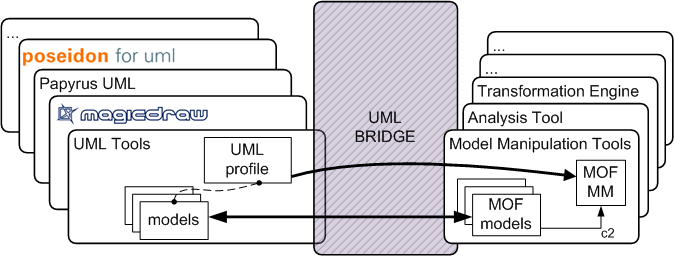
\includegraphics[width=0.85\textwidth]{figures/overview.png}
	\caption{High-level view of the proposed bridge}
	\label{fig:overall}
\end{figure}
\vspace{-.6cm}
Modeling artifacts involved in the bridging procedure lie at different levels of abstraction
(i.e., metamodeling and modeling, in the MDE modeling stack). In order to keep the bridging procedure well defined and manageable,
we decided to keep this distinction in our bridge by decomposing it into two main phases:
%
\vspace{-.1cm}
\begin{itemize}
	\item[$\bullet$] \textbf{phase 1}: it is performed at the metamodeling level, and consists in the generation of $MM$ from the UML profile.
	\item[$\bullet$] \textbf{phase 2}: it works at the modeling level, and consists in the generation of model-to-model
	transformations between UML and $MM$.
\end{itemize}
%
\vspace{-.2cm}
Next sections describe in details the two phases of the bridging procedure.
It is important to note that phases 1 and 2 are executed only once for each UML profile $p_x$, then generated model-to-model transformations
are re-used every time a UML model profiled with $p_x$ has to be bridged.
Furthermore, the proposed bridge is \textit{completely automatic}, i.e., when a UML profile is defined, the above mentioned bridging phases do not require any additional effort to the user. As a matter of fact, designers work on the UML side, while tool developers work on standard MOF metamodels, thus enabling a clear separation of concerns.

\vspace{-.2cm}
\subsection{Phase 1: The bridge at the metamodeling level}\label{sec:metamodelLevel}

At the metamodeling level, the bridge takes an initial UML profile and generates {\em a} corresponding MOF metamodel.
As shown in Figure~\ref{fig:metamodelingLevel}, a model-to-model transformation called
\textit{UMLprofile2MOF} is used for this purpose. This transformation generates a MOF metamodel ($MM_x$ in figure) starting from (i) the definition of the UML profile and (ii) the UML metamodel. The latter input is needed since the transformation has to access UML metaclasses referenced by the various stereotypes of the profile.
%
\vspace{-.4cm}
\begin{figure}[htbp]
	\centering
		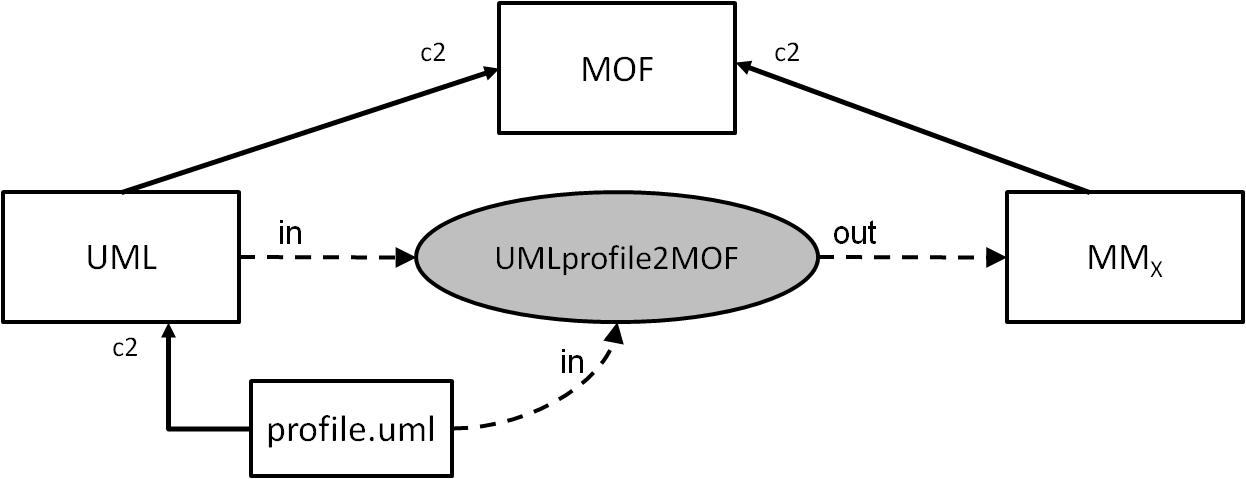
\includegraphics[width=0.60\textwidth]{figures/metamodelingLevel.png}
	\caption{The bridge at the metamodeling level}
	\label{fig:metamodelingLevel}
\end{figure}
\vspace{-.5cm}

%
The \textit{UMLprofile2MOF} transformation contains a transformation rule for each element that can appear in the definition of a UML profile. In the following we describe how the main transformation rules behave:
\begin{itemize}
	\item[$\bullet$] \textbf{Stereotype2Class}. Each UML stereotype is mapped into a MOF metaclass
	(e.g., \textit{XComponent} in Figure \ref{fig:metamodelingExample}).  		
	Tagged values of the source stereotype are separately managed by the \textit{Property2Feature} rule (described below).
	The rule also checks whether the source UML stereotype specializes some other elements, and recreates the generalization hierarchies in the target MOF metamodel, accordingly.
	A special reasoning is applied to transform the relationship between a stereotype and the UML metaclasses it extends.
	According to the UML superstructure~\cite{UML}, \textit{"the MOF construct equivalent to an extension is an aggregation from
	the extended metaclass to the extension stereotype"}. So, this rule transforms each UML extension into
	a MOF containment reference with cardinality \textit{0..1}. 	
	\item[$\bullet$] \textbf{Class2Class}, each UML class is mapped to a MOF metaclass.
	Properties of the source UML class are managed by the \textit{Property2Feature} rule and, similarly to \textit{Stereotype2Class},
	contains a mechanism for managing its generalization hierarchy.
	\item[$\bullet$] \textbf{Profile2Package}, each UML profile is mapped to a MOF package (e.g.,the \textit{ XProfile} in figure). Specific bindings populate the newly generated package with the correct metaclasses (generated either by the \textit{Class2Class} or the \textit{Stereotype2Class} rules) in order to recreate the same hierarchy of containments.
	\item[$\bullet$] \textbf{Package2Package}, each UML package is mapped to a MOF package. It is populated in a similar way as in the \textit{Profile2package} rule.
	\item[$\bullet$] \textbf{Property2Feature}, each UML property (like the \textit{executionTime} in figure)
	is mapped to a MOF attribute or reference depending on their type;
	more specifically, if the type of the source property is either a data type, an enumeration or a primitive type,
	then a MOF attribute is generated, otherwise the rule generates a MOF reference.
	\item[$\bullet$] \textbf{DataType2Datatype}, each UML data type is mapped to a MOF data type.
	\item[$\bullet$] \textbf{Enumeration2Enumeration}, each UML enumeration (\textit{type} in figure)
	is mapped into a MOF enumeration containing the same literals.
\end{itemize}
%
\vspace{-.8cm}
\begin{figure}[htbp]
	\centering
		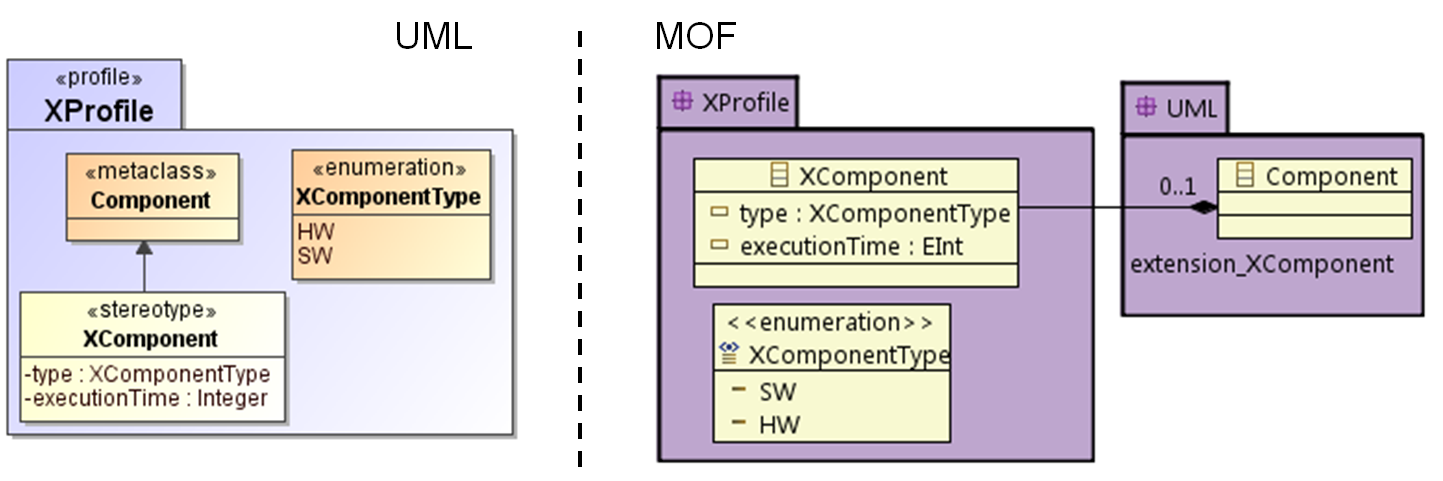
\includegraphics[width=0.70\textwidth]{figures/metamodelingExample.png}
	\caption{Example of generated MOF metamodel}
	\label{fig:metamodelingExample}
\end{figure}
\vspace{-.6cm}

\textit{UMLprofile2MOF} also contains a set of auxiliary rules and bindings (e.g., the one setting the name of each MOF meta-element with the name of the corresponding source UML element, etc.), not described in this paper for sake of simplicity. Furthermore, \textit{UMLprofile2MOF} creates an ad-hoc package in $MM_x$ where it copies all the UML metaclasses in there. In this way, the generated MOF metamodel is self-contained, and does not depend on the UML metamodel itself.
%; this opens for the possibility to "slice" the MOF metamodel, allowing to do not suffer from the complexity of the UML metamodel any more.This aspect of the bridge is presented in Section~\ref{sec:slicing}.

%Figure \ref{fig:metamodelingExample} represents a trivial UML profile translated into a MOF metamodel. The Profile has been translated into a MOF package, the Component metaclass has been copied to the target metamodel and extended through the \textit{extension\_MyStereotype} attribute. Eventually the Stereotype has been translated into a MOF metaclass and bound with the extended metaclass by means of the composition reference.
%%
\vspace{-.2cm}
\subsection{Phase 2: The bridge at the modeling level}\label{sec:modeLevel}

At the modeling level, the proposed bridge automatically generates model-to-model transformations between UML profiles and MOF metamodels.
More specifically, Figure~\ref{fig:modelingLevel} shows the two model transformations generated by our bridge:
%
\vspace{-.1cm}
\begin{itemize}
	\item $UML2MM_x$ returns a model conforming to $MM_x$, starting from a UML model conforming to the $profile.uml$ profile;
	\item $MM_x2UML$ performs the opposite task: it takes as input a model conforming to $MM_x$
	and produces UML models profiled according to $profile.uml$.
\end{itemize}
%
\vspace{-.4cm}
\begin{figure}[htbp]
	\centering
	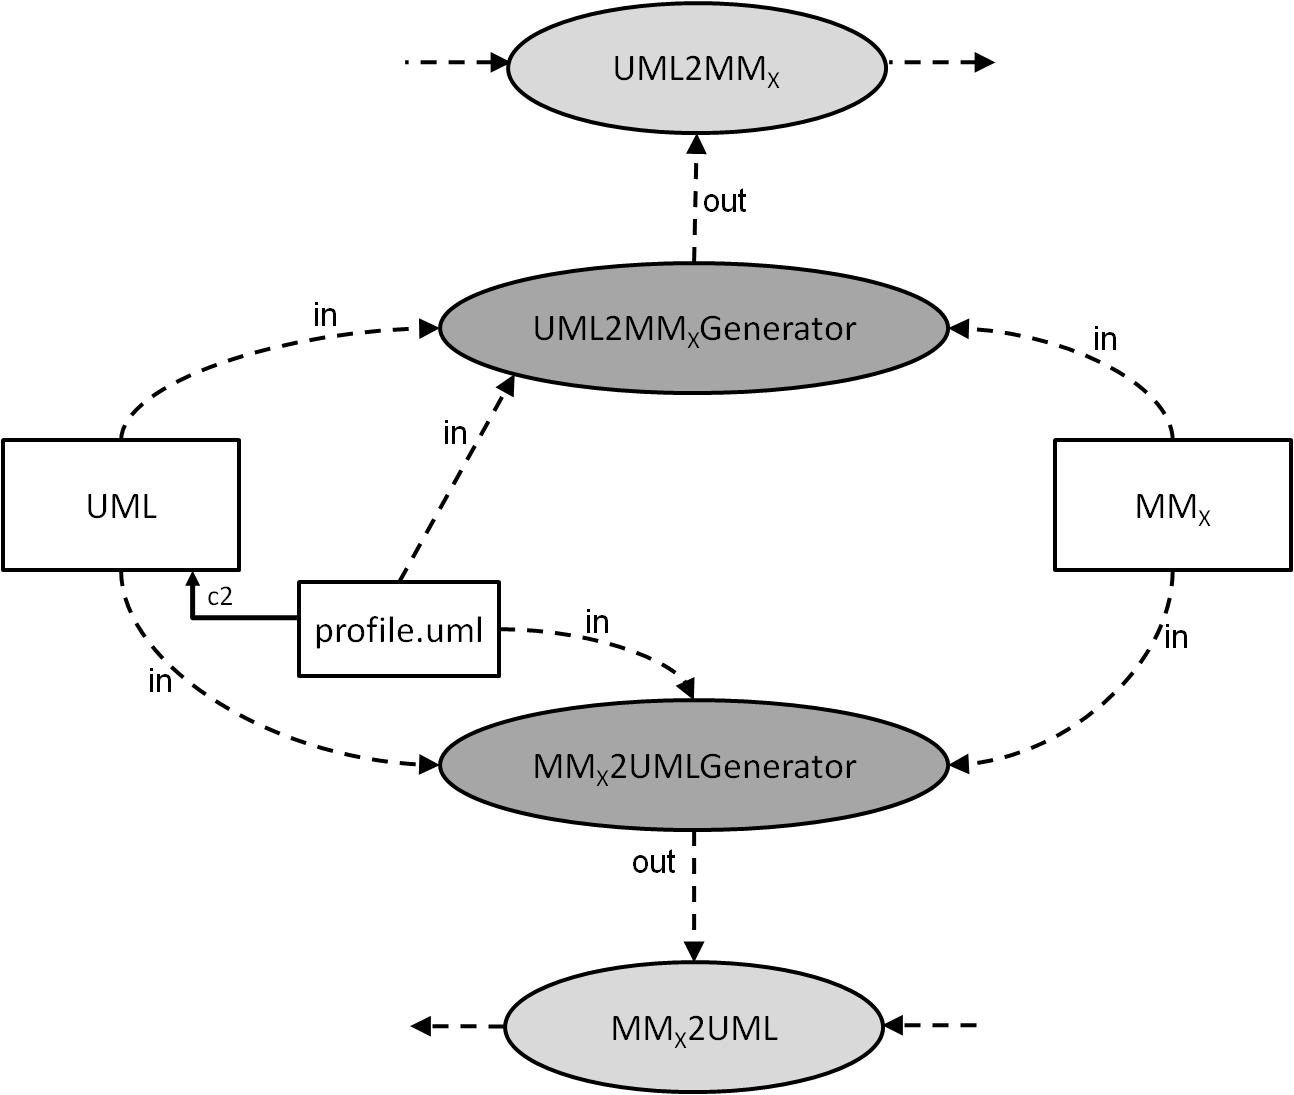
\includegraphics[width=0.60\textwidth]{figures/modelingLevel.png}
	\caption{The bridge at the modeling level}
	\label{fig:modelingLevel}
\end{figure}
\vspace{-.4cm}

$UML2MM_x$ has the following high-level logical structure: (i) a set of rules transform each standard UML element into an instance of its corresponding metaclass in $MM_x$; (ii) another set of rules transform each stereotype in the UML profile into an instance of the corresponding metaclass in $MM_x$; and (iii) for each rule, some imperative code is generated in order to automatically manage the application of stereotypes. $MM_x2UML$ works in the other way round: (i) firstly it applies the UML profile to the target UML model; (ii) then, it transforms each instance of metaclasses in $MM_x$ into an instance of the corresponding UML element; (iii) stereotypes are applied to  previously generated elements according to the definition of the UML profile. Specific rules manage the order in which profiles and stereotypes are applied, and how tagged values are accessed in the models. Figure~\ref{fig:modelingExample} shows an example of models produced by the bridge.
%
\vspace{-.4cm}
\begin{figure}[htbp]
	\centering
		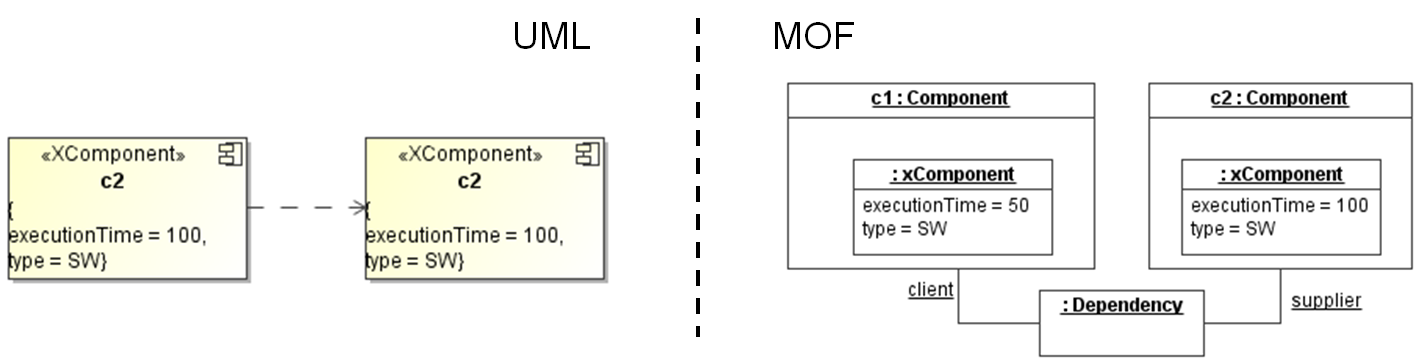
\includegraphics[width=0.70\textwidth]{figures/modelingExample.png}
	\caption{Example of bridged models}
	\label{fig:modelingExample}
\end{figure}
\vspace{-.8cm}

Such transformations are automatically generated by means of the execution of two Higher-Order Transformations
(i.e., transformations taking other transformations as input or producing
other transformations as output): $UML2MM_xGenerator$ and $MM_x2UMLGenerator$. It is important to note that higher-order transformations make the bridge generic (and so, totally automatic), so that it does not depend neither on source UML profiles nor on the generated MOF metamodels.
%In the figure \ref{fig:modelingExample} we show the result of the execution of the generated transformation on a model which has applied a the example profile of figure \ref{fig:metamodelingExample}. As you can see the element is a \textit{Component} and has applied \textit{MyStereotype} stereotype. In the target model we have an instance of a \textit{Component} MOF class which has an instance of a \textit{MyStereotype} class. Every tagged value has been kept and rightly instantiated.


%------------------------------------------------------------------------------------------------------------------------
\section{Slicing the obtained metamodel}\label{sec:slicing}

The default behavior of the bridge is to consider the whole UML metamodel and to keep its concepts also in the
target MOF metamodel. While ensuring loss-less transformation (and this is our primary goal while designing the bridge), our current 
approach moves the complexity of the UML metamodel (containing 246 classes and 583 properties)
into the target MOF metamodel. In order to avoid such a complexity, we couple the bridge with a \textbf{slicing mechanism} that reduces the generated metaclasses to a \textit{subset of relevant UML concepts}.

The subset of relevant UML concepts can be considered as the set of metaclasses that are expected to be instantiated
in the context of a specific project; metaclasses outside the relevant set are never instantiated in any model.
A typical example is when designers assume that they will only use, e.g., use case diagrams.
In this scenario, relevant UML concepts are only those pertaining to use case diagrams (e.g., actor, use case, association)
and there is no need to keep modeling concepts for state machines, sequence diagrams, and so on.
%This kind of assumptions is recurrent in practice, thus we designed our approach so that the target MOF metamodel contains only
%metaclasses corresponding to relevant UML concepts.
%indeed many UML modeling tools allow to restrict the kind of diagrams that can be created by designers.
%
%\begin{wrapfigure}{l}{0.45\textwidth}
	%\vspace{-20pt}
	%\begin{center}
	%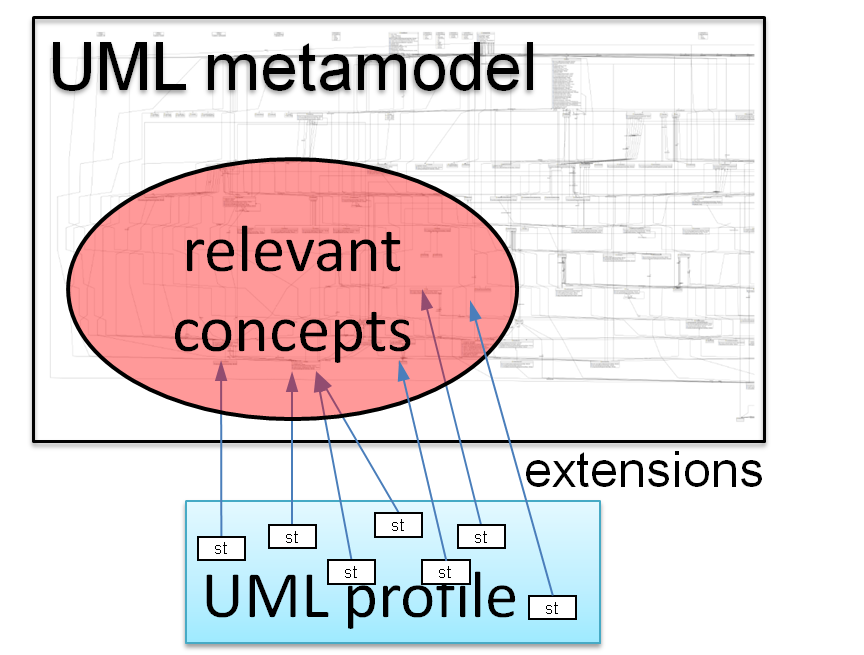
\includegraphics[width=0.44\textwidth]{figures/slicingIdea.png}
	%\end{center}
	%\caption{UML relevant concepts}
	%\label{fig:slicingIdea}
	%\vspace{-20pt}
%\end{wrapfigure}
\begin{figure}
  \centering
  \subfloat[from the UML profile]{\label{fig:slicingIdea1}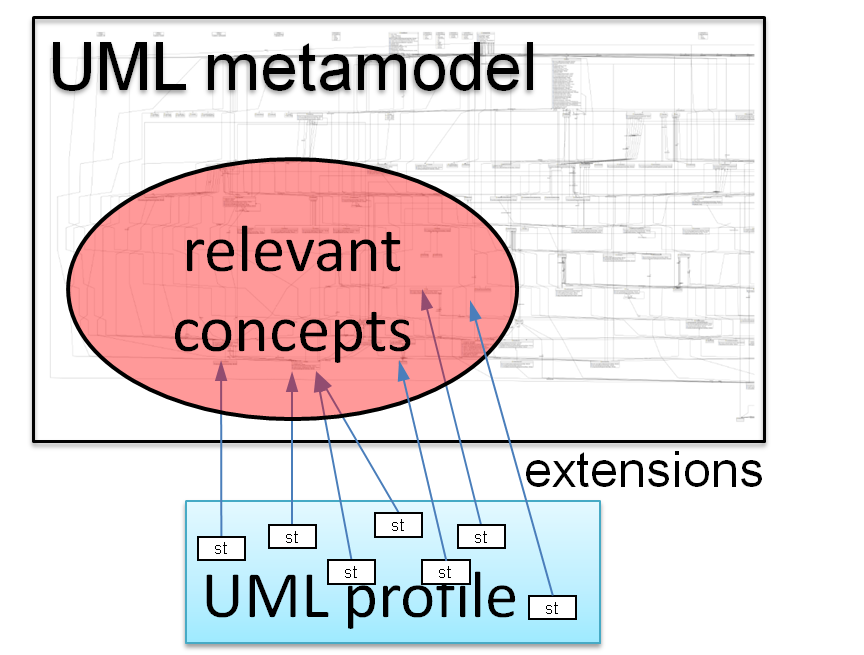
\includegraphics[scale=0.255]{figures/slicingIdea.png}}
	\hspace{2mm}
  \subfloat[from diagram names]{\label{fig:slicingIdea2}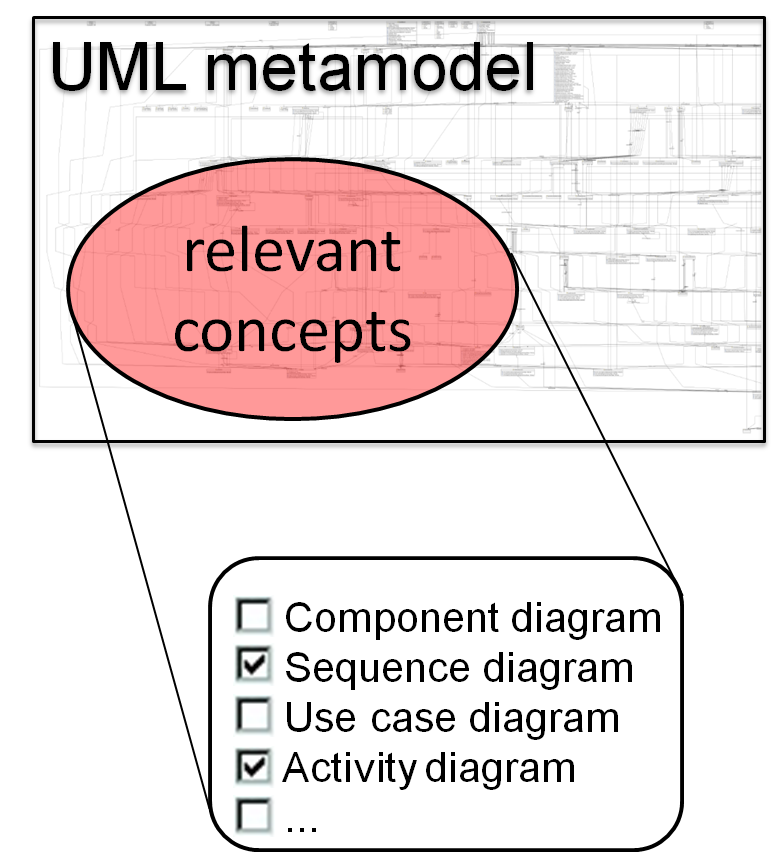
\includegraphics[scale=0.255]{figures/slicingIdea2.png}}
	\hspace{2mm}
  \subfloat[from example models]{\label{fig:slicingIdea3}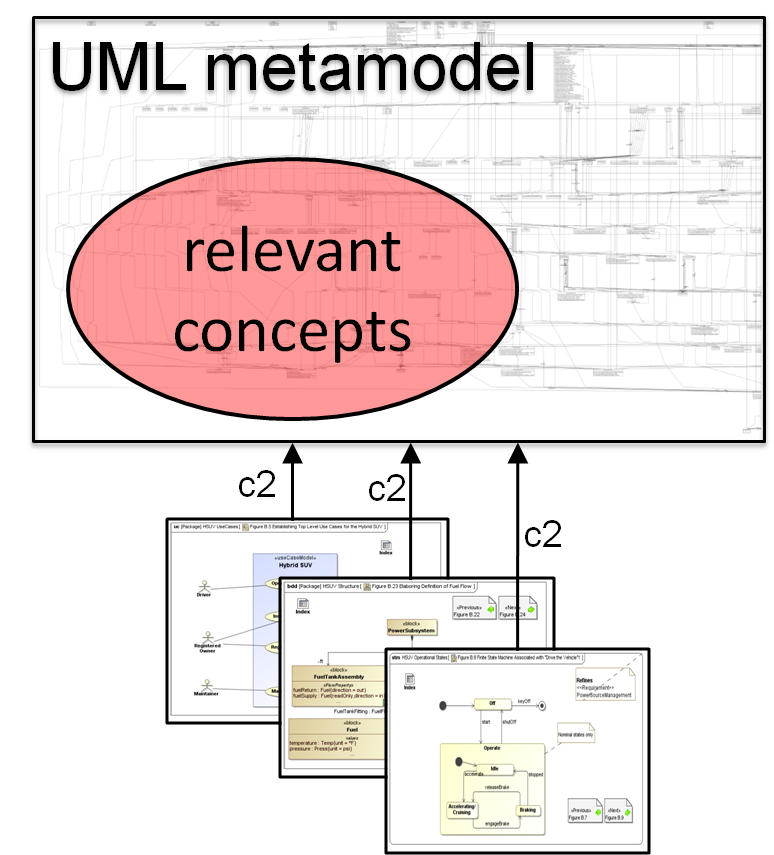
\includegraphics[scale=0.255]{figures/slicingIdea3.png}}
  \caption{Mechanisms for defining the set of UML relevant concepts}
  \label{fig:slicingIdea}
\end{figure}
%
The remainder of the section is organized as follows: firstly we describe the slicing algorithm, then we describe how sets of relevant UML concepts can be represented as annotation models, and then we will discuss how the slicing algorithm can be executed on both the target MOF metamodel and the generated model transformations.

\textbf{Slicing algorithm}. Once a set of relevant UML concepts is identifies, the slicing mechanism can be applied. Our proposal
is based and extends a generic slicing algorithm for MOF metamodels presented in~\cite{ICSEbyadl}. Intuitively,
it considers the set of relevant metaclasses and then navigates both their references and generalizations in order
to return a self-contained subset of the initial metamodel.
More formally, let $MM$ be a metamodel and let $SC$ be a subset of relevant elements in
$MM$; $slice$ is defined as follows:

\vspace{-.2cm}
$$slice(SC)=SC \cup \displaystyle\bigcup_{c \in
SC}{slice(neighbour(c))}$$
\vspace{-.2cm}

\noindent where $neighbour(c)$ is the set of all super metaclasses of
$c$, of all metaclasses referred (both with association and
aggregation) by $c$, and of all types of attributes in $c$.
It is important to note that even though $slice$ is defined
as a set of metaclasses, since each metaclass contains also references
to other metaclasses, the final result is a subset of the metamodel $MM$
with both metaclasses and their meta-relations. In this work we modified the original slicing algorithm in two ways:
(i) we implemented it as a reusable library for model-to-model transformations (previously it was embedded into
the tool itself), and (ii) we introduced specific helpers to manage UML-specific issues (e.g.,
every UML model must contain a root element called \texttt{Model}, so we added a specific helper that ensures that the slicing
algorithm does not leave out this root element from the target MOF metamodel).

%The set of relevant metaclasses is an information related to the target MOF metamodel but it is not included in it (it depends on specific needs of designers).
\textbf{Annotation models}. Since the slicing mechanism is realized as a model transformation, the set of relevant metaclasses is represented as an \textit{annotation model}
\footnote{An annotation model is a model containing auxiliary information about another model (the annotated model)\cite{MCDFthesis}} linked to the target MOF metamodel.
The annotation model contains a link to each relevant metaclass coming from UML: the slicing mechanism uses those links to identify the initial set of metaclasses that will not be sliced out by the slicing procedure.
The current version of the bridge provides three mechanisms to (semi) automatically obtain the annotation model that will drive the slicing procedure:
%
\begin{enumerate}
	\item the annotation model is automatically generated from a UML profile (Figure \ref{fig:slicingIdea1}); intuitively, it creates a link in the annotation model
	for each UML metaclass extended by at least a stereotype in the profile.
	\item the GUI of the bridge allows designers to specify only the types of UML diagram they will use (e.g., activity, sequence diagrams), and the corresponding annotation model
	is automatically generated (Figure \ref{fig:slicingIdea2}); basically, designers provide the names of the UML diagrams, and this mechanism deduces the set of metaclasses belonging to those diagrams, then a link for each of those metaclasses is created in the annotation model.
	\item designers provide an example of a UML model, and then the annotation model is automatically generated from it (Figure \ref{fig:slicingIdea3}).
	Basically, this mechanism checks which metaclasses are instantiated in the example model and creates a link for each metaclass found in the annotation model.
\end{enumerate}
%
These mechanisms are implemented as model transformations. Each mechanism has a different level of automation and requires different input artifacts. For example, if designers already know they will use only specific UML diagrams, then option 2 may be the most convenient;
or else, if designers already defined some initial model, they may use option 3.
Of course, if full control over the generated metamodel is needed, designers can manually define the annotation model by means of a dedicated graphical editor.
Furthermore, those mechanisms can be executed incrementally; for example a metamodel could be sliced by means of
mechanism 1, and then the resulting metamodel could be sliced multiple times with mechanism 3 with different example models:
the resulting metamodel will be more concise and accurate.
%that is they can create an annotation link for each metaclasses that can be instantiated in their UML models.
%
\vspace{-.4cm}
\begin{figure}
  \centering
  \subfloat[]{\label{fig:slicerMM}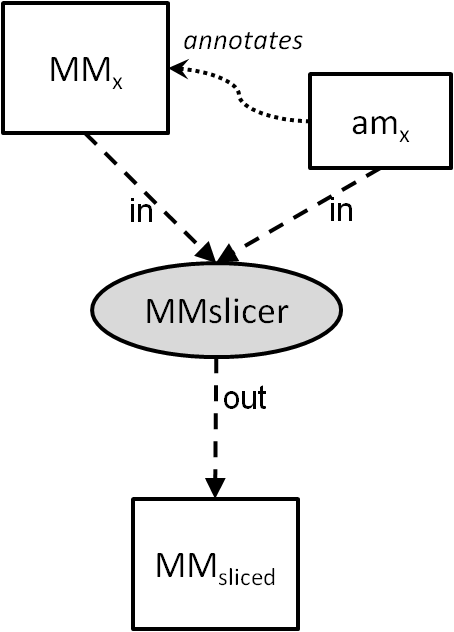
\includegraphics[scale=0.4]{figures/slicerMM}}
 \hspace{10mm}
  \subfloat[]{\label{fig:slicerT}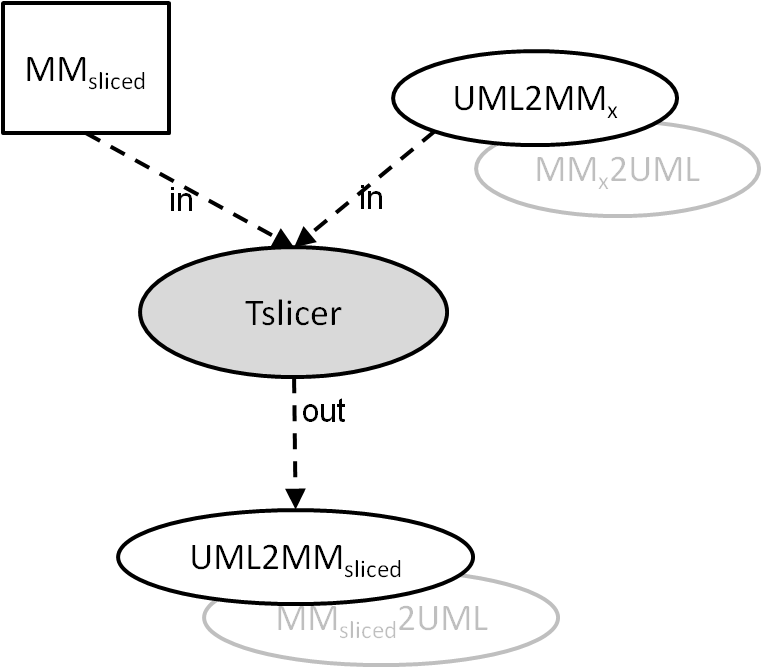
\includegraphics[scale=0.4]{figures/slicerT.png}}
  \caption{Slicing the MOF metamodel (a) and the generated transformations (b)}
  \label{fig:slicer}
\end{figure}
\vspace{-.4cm}

\textbf{Slicing metamodels}. As can be seen in Figure \ref{fig:slicerMM}, the slicing algorithm is used at the M2 level by a model-to-model transformation called \textit{MMslicer}.
It takes as input a MOF metamodel $MM_x$ and an annotation model $am_x$, and generates a new metamodel $MM_{sliced}$.
The resulting metamodel is self-contained (i.e., it does not contain any reference to external metamodels)
and contains a subset of $MM_x$ according to the metaclasses referenced in $am_x$.

A possible issue that may arise needs to be discussed: once the target MOF metamodel has been sliced, the
previously generated model transformations implementing the bridge may refer to missing metaclasses in the metamodel.
For example, if all the concepts related to state machines have been sliced out, the generated $UML2MM_x$ transformation still contains
transformation rules for transforming states, transitions, etc.; so, it is not aligned with the newly sliced metamodel and its execution will be erroneous.
This implies that our approach has to provide a mechanism for adapting also the $UML2MM_x$ and $MM_x2UML$ transformations
to the newly sliced metamodel.
We are aware that in literature there are generic approaches managing the coupled evolution of metamodels and model transformations
\cite{TransEvolution}; however, since in our approach elements
can be only deleted from metamodels (neither added nor updated), and since we need a fully automatic mechanism, we developed our minimalistic solution to automatically adapt model transformations to sliced metamodels.

\textbf{Slicing transformations}.
Our solution takes inspiration from the EMFMigrate project\footnote{EMFMigrate project website: \small{\url{http://www.emfmigrate.org}}}
and is based on an higher-order transformation; in this work we call it $Tslicer$.
%This kind of issue is well-known in the metamodel co-evolution research field \cite{CITAZIONI}, \footnote{http://www.emfmigrate.org}
Figure \ref{fig:slicerT} gives an idea of how the \textit{Tslicer} transformation works. It takes as input (i) the sliced metamodel
($MM_{sliced}$ in figure) and (ii) the model transformation to be adapted ($UML2MM_x$ in figure). $Tslicer$ automatically adapts the input transformation according to the meta-elements (i.e., metaclasses, attributes, references) that were previously sliced out from $MM_{sliced}$.
Basically, it traverses all the instructions of the input transformation (e.g., transformation rules, assignments)
and deletes those instructions referring to meta-elements not contained into the $MM_{sliced}$ metamodel.
The grey elements in Figure \ref{fig:slicerT} show that $Tslicer$ can also be
applied on the transformation in the other direction (i.e., $MM_x2UML$); this ensures that using the slicing mechanism does not affect
the bridge in terms of automation and bidirectionality.
%The interested reader can refer to  details on $Tslicer$ are provided in Section \ref{sec:tool}.

In conclusion, it is important to note that the whole slicing mechanism (both on metamodels and transformations)
acts as a post-processing activity of the artifacts generated by the bridge described in Section \ref{sec:framework}; this means that, according to project-specific needs, the proposed bridge and slicing mechanism can be used independently.

%\henry{Una cosa: perche' invece di generare prima il metamodello e poi applicarci lo slicing, non generiamo direttamente un metamodello sliced? Se capisco bene, cio' ci eviterebbe di applicare l'ultimo passo qui descritto. Se e' nei future work, diciamolo da qui.}
%Intuitively, it copies all the elements of the input transformation (like transformation rules, imperative statements, conditions, and so on)
%and ignores those elements that reference a meta-element  that are not in $MM_sliced$ anymore.

%removes those elements of the input model transformation (e.g., transformation rules, imperative statements, conditions)
%that reference a meta-element that is not in $MM_sliced$ anymore (i.e., such an element has been sliced out by $Mslicer$).

\section{Implementation of the bridge}\label{sec:tool}
We implemented the proposed bridge in the context of the Eclipse platform.
More specifically, it is realized as an Eclipse plugin that can be used in two different ways: i) as a standard Eclipse plugin: this allows designers to integrate the bridge with other technologies available in the Eclipse community (e.g., model differencing tools, model transformation engines, and so on); ii) as a stand-alone application in which the bridge and its dependencies are packed together: this allows designers to use the bridge also outside the Eclipse environment.

%Figure~\ref{fig:tech} shows the modeling technologies we used to realize the bridge (for the sake of simplicity,
%transformations from MOF to UML are not represented in figure). 
In our approach, models and metamodels are represented by means of the EMF
framework\footnote{EMF project website: \small{\url{http://www.eclipse.org/modeling/emf/}}}.
It includes an implementation of the MOF meta-metamodel called Ecore, and runtime support for models including,
among all, persistence support by serializing models in the OMG XML Metadata Interchange (XMI).
UML profiles are defined using UML2,
the implementation of the UML metamodel for the Eclipse
platform\footnote{UML2 project Web site:
\underline{http://www.eclipse.org/uml2/}.}.
This provides the bridge full compliance with OMG standards
(specifically UML 2.0 and MDA) and interoperability with other
UML modeling tools\footnote{List of UML2-compatible UML Tools: \small{\url{http://wiki.eclipse.org/MDT-UML2-Tool-Compatibility}}}. Thanks to this choice, designers can graphically design UML profiles with any UML modeling tool, and directly import them into
the Eclipse environment. The same rationale holds for UML models.
%
%\begin{figure}[htbp]
%	\centering
%		\includegraphics[width=0.80\textwidth]{figures/implementation.png}
%	\caption{Modeling technologies for the realization of the bridge}
%	\label{fig:tech}
%\end{figure}

Both model transformations and annotation models are based on the Atlas Model Management Architecture (AMMA)~\cite{1}.
More specifically, the model transformations constituting the bridge are specified using the
Atlas Transformation Language (ATL)~\cite{3}, a hybrid model transformation language with both declarative and imperative constructs (Listing \ref{lst:generatedTransf} shows an excerpt of ATL code).
The technology used for representing and manipulating annotation models is the Atlas Model Weaver (AMW)~\cite{3}. It allows the (graphical) definition of correspondences
among models and links among model elements. Such links are captured by weaving models conforming to an extensible weaving metamodel~\cite{MCDFthesis}. The AMMA platform has been selected since it best fits the requirements required to implement the bridge: (i) it provides a flexible model transformation engine, (ii) it supports the concept of transformation model, thus enabling the development of higher-order transformations, and (iii) it is integrated into Eclipse and its modeling facilities~\cite{bezivin_06_canonical}.

Interested readers can download the current version of the bridge (along with its source code) from the project
web page at \small{\url{http://www.di.univaq.it/malavolta/umlbridge}}.





\section{Case study}\label{sec:caseStudy}
In this section we show the application of the proposed UML bridge to a non-trivial case study based on the SysML profile.
SysML is a general-purpose modeling language for systems engineering applications \cite{sysml}, it has been proposed by the OMG group
and supports the specification of  hardware, software, processes, and facilities of a system.
The objective of this case study is to present how each aspect of the proposed approach works in practice on SysML models.

\begin{figure}[htbp]
	\centering
		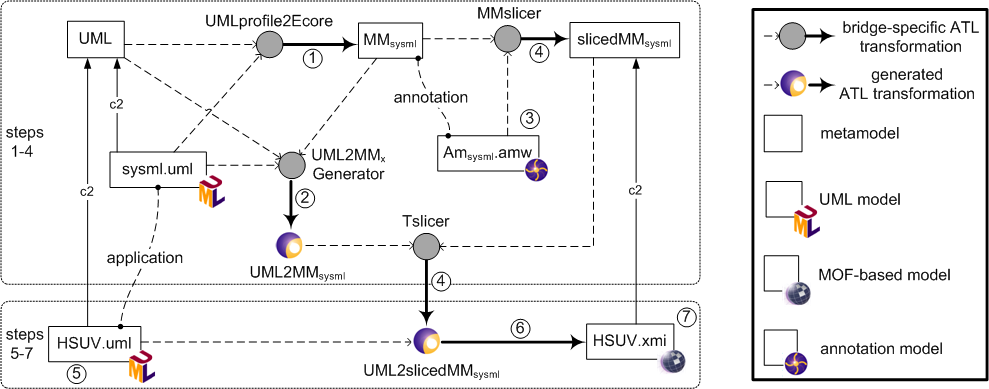
\includegraphics[width=1\textwidth]{figures/caseStudy.png}
	\caption{Overview of the HSUV case study}
	\label{fig:caseStudy}
\end{figure}

As shown in Figure \ref{fig:caseStudy}, we organized the case study as a seven-steps process:
%
\begin{enumerate}
	\item transformation of the SysML profile into a MOF metamodel called $MM_{sysml}$;
	\item automatic generation of the model transformation that creates MOF-based models from SysML-profiled models;
	\item creation of an annotation model $am_{sysml}$ to slice $MM_{sysml}$;
	\item execution of \textit{MMslicer} and \textit{Tslicer} according to the $am_{sysml}$;
	\item design of a SysML-profiled UML model ($HSUV.uml$ in figure);
	\item transformation of $HSUV.uml$ into its MOF-based counterpart ($HSUV.xmi$);
	\item development of a simple manipulation tool that works on $HSUV.xmi$.
\end{enumerate}
%
Before going into the details of each step, it is important to note that steps 1-4 are executed only once for each
UML profile to bridge (SysML in this case), then the generated ATL transformation 
can be re-used every time a profiled UML model has to be bridged.

\ivano{dire che due to space limitations non mettiamo le cose che valgono a livello metamodello, ma ci focalizziamo sui modelli e la trasf finale.}

In this case study we use the Papyrus modeling tool\footnote{Papyrus UML web site: \small{\url{http://www.papyrusuml.org}}} as UML
tool. We chose it for two main reasons: (i) a SysML add-in provides support for modeling SysML-like models in Papyrus according to
the official SysML specification,
and (ii) it is based on Eclipse, so our bridge and the Papyrus tool coexist in the same modeling environment.

\textbf{Step 1.} We firstly consider the SysML profile definition made available by the Papyrus add-in,
and then we transform it into the corresponding MOF metamodel
by means of the $UMLprofile2MOF$ transformation (it is described in Section \ref{sec:metamodelLevel}). 
The resulting $MM_sysml$ metamodel is composed of XX metaclasses, YY attributes and ZZ references 
(either associations, aggregations or generalizations).

\textbf{Step 2.} In this step we execute the higher-order transformation called $UML2MM_xGenerator$ in order to obtain the
model transformation that takes as input SysML-profiled models and returns MOF-based models. The generated transformation 
($UML2MM_{sysml}$ in figure) is composed of XXX transformation rules, YYYY feature bindings, ZZZ helpers; the total size of the transformation is XXXX lines of ATL code.

\textbf{Step 3.} In order to slice the obtained metamodel and transformation, 
we (automatically) generate an annotation model by means of the second generation mechanism
(see Section \ref{sec:slicing}) by assuming that only XXX and YYY diagrams are used.
The generated annotation model ($am_{sysml}$ in figure) contains XXXX links to metaclasses like YYY, XXX, and so on.

\textbf{Step 4.} The newly created annotation model is used to execute the \textit{MMslicer} and \textit{Tslicer} transformations.
These transformations adapt $MM_{sysml}$ and $UML2MM_{sysml}$ by leaving out those elements that do not belong either to XXX or YYY diagrams. 
The adapted metamodel ($slicedMM_{sysml}$) contains XXX metaclasses, yy attributes and ZZ references. 
The size of the adapted transformation ($UML2slicedMM_{sysml}$) is XXXX lines 
of ATL code; it contains XXX transformation rules, YYYYY feature bindings and ZZZ helpers. 
The $UML2slicedMM_{sysml}$ transformation will be used to transform the initial UML model described in the next step into its 
corresponding MOF-based model.

\textbf{Step 5.} In order to XXX, we decided to reuse an already existing SysML-based UML model. So we in this case study we consider
 the example model provided in the SysML official specification and we developed it in the papyrus modeling tool.
This model represents a Hybrid gas/electric powered Sport Utility Vehicle (HSUV) by focussing on its requirements, performance, structure, and behavior. Figure \ref{fig:hsuvUML} shows a fragment of ..... \ivano{completare}. Due to space limitations, we do not provide the details of the HSUV model, however the interested reader can download and use the full UML model from our UML bridge web page. 

\begin{figure}
  \centering
  \subfloat[]{\label{fig:hsuvUML}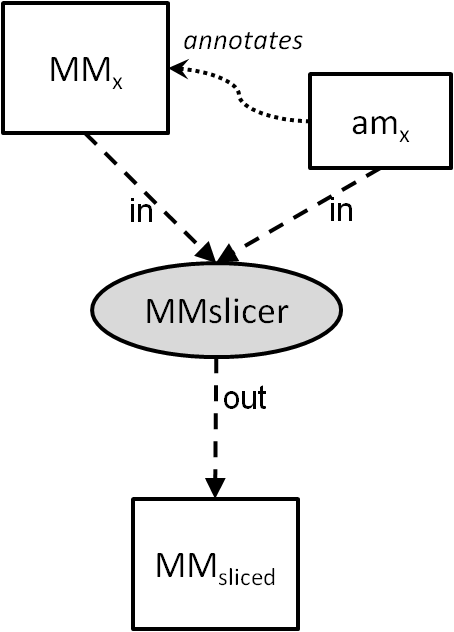
\includegraphics[scale=0.4]{figures/slicerMM}}
 \hspace{10mm}
  \subfloat[]{\label{fig:hsuvMOF}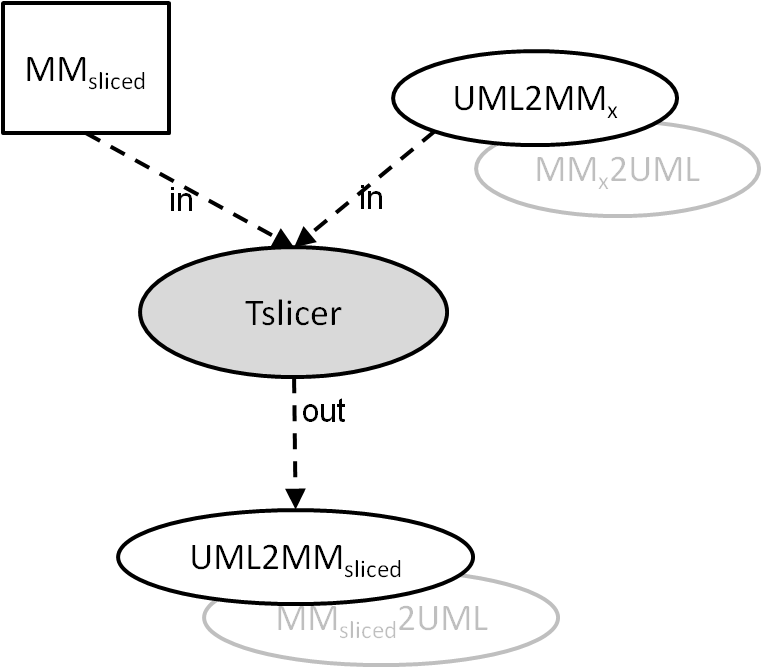
\includegraphics[scale=0.4]{figures/slicerT.png}}
  \caption{HSUV system: a UML model (a) and its corresponding MOF-based model (b)}
  \label{fig:hsuv}
\end{figure}
%
\textbf{Step 6.} At this point we can execute the $UML2slicedMM_{sysml}$ Transformation in order to obtain a MOF-based representation
of the HSUV model. Figure \ref{fig:hsuvMOF} shows a fragment of the .... \ivano{completare}.

\textbf{Step 7.} In this step we provide an extremely simplified manipulation tool that operates on bridge MOF models. 
It is important to point up that technical accuracy and XXX are not in the focus of this part of the case study, 
its main goal is to show as clearly as possible how manipulation tools may benefit from our UML bridge. 
More specifically, the manipulation tool is implemented as an ATL transformation that XXXX...
%
\begin{lstlisting}[breaklines,style=AMMA,language=ATL,mathescape,rulesepcolor=\color{black},caption=ATL transformation working on MOF-based SysML models,captionpos=b,label={lst:manipulationTool}]
helper context OclAny def : UntypedGenericKernels : 
  Set(GenericKernel) = 
  MM!GenericKernel.allInstancesFrom('IN')
    ->select(x | x.type.oclIsUndefined());
...
entrypoint rule KernelTypeUpdate {
  do {
    for (e in thisModule.UntypedGenericKernels()) {
      e.type<-thisModule.createNewKernelType(e);
      thisModule.setSuperTypes(e.type);
      ...
}}}
\end{lstlisting}

Listing \ref{lst:manipulationTool} shows an excerpt of this transformation. 
\ivano{il dominio della trasf e' piccolo e ben definito, accedere agli stereotipi e' piu facile, accedere ai valori dei tagged value e' piu facile}



%The objective of this case study is to present how the UML bridge works at both metamodeling and modeling
%abstraction layers, how the slicing mechanism works in practice, and how a XXX manipulation tool may benefit from
%the application of our approach.
\section{Related work}\label{sec:related}
\ivano{descrizione di lavori simili in letteratura e come si differenziano da noi}

\ivano{mini intro}

The problem of bridging between UML profiles and metamodels has already been addresses in previous researches. Abouzahra, B\`ezivin et al. \cite{Abouzahra}, propose an integration process starting from a UML profile and a MOF metamodel. 
The tool, they implemented, takes as input an UML profile and the metamodel of the system described by the profile. That tool allows
transforming between models conforming to those inputs. It transforms UML models designed with this profile to models conforming to the profiled metamodel and vice versa. The tool aims at automatically generating transformations between models and not transforming a metamodel to a profile or the opposite. To reach this goal it needs mapping links to be implemented. Mapping details specify links between UML elements and the elements from the profiled metamodel. This information should not to be redundant. To meet this requirement, this approach represents the two input models (the profile model and the profiled metamodel) separately. A modeling weaving tool, the AMMA model weaving one, has been used for this purpose. This approach has the limitation of finding correspondences between the profile and the metamodel, as mentioned in the limitation section of their paper, since there's no normalized way to define UML profiles and their mapping with MOF metamodels. What we propose is a tool wich bridges, in a completely automated manner, a profile to metamodels (and every profiled model into the corresponding). This previous approach led us the way to our approach.

Another approach has been proposed by Manuel Wimmer in this \cite{Wimmer}. Assuming there's no available profile yet, this approach proposes a Bridge Generator component which automatically generates transformations and profile by means of an explicit, and manually build, mapping model. The integration process then is as follows: First, the user defines the correspondences between the DSL metamodel and the UML metamodel in terms of a mapping model in an interactive mapping environment. The mapping model is expressed with a dedicated metamodel bridging language which enables the automatic processing. After finalizing the mapping model, the Bridge Generator automatically generates the UML profile and in the case that an uni-directional model transformation language is used, also the transformations from the DSL to UML and back again. Wimmer's approach has, as its principal benefit, the reduction of error having a single source of information (the mapping model) and automated repetitive tasks by means of the transformation. Our approach, again, has the completely automated manner of defining the mapping. Moreover, our approach is in a way specular to Wimmer's one, since our starting point is a profile and several profiled models.

Another method used for bridging purposes is the use of EMF umlutil.java library. This library converts UML elements to representative Ecore model elements. This utility helps, in the Eclipse framework, to automatically convert UML elements into Ecore ones. Nevertheless the conversion is possible only at the metamodeling level, one developer has to manually implement transformations from his own profile to the metamodel that is the strenght of the bridge we are propose here.

\marco{reference al sito? http://download.eclipse.org/modeling/mdt/uml2/javadoc/2.2.0/org/eclipse/uml2/uml/util/UMLUtil.UML2EcoreConverter.html}
\section{Conclusions}\label{sec:conclusion}
In this paper we presented an automatic bridge between UML profiles and MOF metamodels.
The problem that we want to alleviate is due to the fact that, even if profiled UML models are very used since they are intuitive for designers and model editors already exist, 
they are intrinsically complex for model manipulation.
So, the main goal of the proposed bridge is to support those kind of projects in which the system is modelled using UML profiles, and there is a strong need of automatic model manipulation.

The bridge is fully automatic and
%, unless designers do not make particular assumptions on the models 
%(see the slicing mechanism), 
loss-less with respect to the information provided in the models. 
These two aspects make the use of the proposed bridge totally transparent for designers, allowing
model manipulation tool developers to gain from its features. The bridge is coupled with a slicing mechanism
that allows to obtain smaller and more concise target MOF metamodels.
In order to test its capabilities, we applied the proposed bridge to a non-trivial and widely used profile:
SysML. 

If on one side the application to a real-sized profile provided interesting insights and proved the usefulness of the bridge, on the other side it unveiled some of its \textbf{\textit{limitations}}.
For example, the current implementation of the bridge is able to manage nested profiles (i.e., profiles containing other profiles), but it
cannot manage profiles referencing external profiles.
Furthermore, the slicing mechanism for model transformations can be enhanced in different ways. For example, currently it deletes all the
elements (e.g., transformations rules, feature bindings, etc.) referring to meta-elements that have been sliced out from the metamodel;
this behavior is correct and straightforward to be implemented, but we also recognize that it is a basic solution 
and something more elaborated should be provided. \ivano{other limitations?}

The primary \textbf{\textit{future work}} direction for our UML bridge is to overcome the above mentioned limitations.
Furthermore, we are also studying how to customize the generation of the target MOF metamodel by deciding a priori the number of levels in its generalizations hierarchy, by specifying whether or not some kind of attributes should be part of it or, more in general, to specify a priori some kind of characteristics that
the target MOF metamodel must have. 
We are also planning to evolve the slicing mechanism by providing a richer annotation model; for example,
designers can define a kind of black-list of meta-elements that must not be part of the sliced metamodel. 
%Another interesting research direction concerns
%the study of a mechanism for analyzing the UML "metamuddle" and then to automatically return a kind of \textit{simpleUML} metamodel with an higher-level of abstraction than UML. 
Moreover, we are planning to study our bridge in the context of model-based analysis and to check
how the proposed bridge can be combined with regression analysis techniques.
In conclusion, we are planning to embed the bridge in stable releases of other research tools; this gives us two main benefits:
(i) on one side those research tools will benefit from the features of the UML bridge, 
(ii) on the other side it also gives us the possibility to continuously test (and enhance) the UML bridge itself.




%\section*{Acknowledgments} This work is partly supported by the
%EU IST CONNECT ({\small\url{http://www.connect-forever.eu}}) No
%231167 of the FET - FP7 program and the Italian PRIN d-ASAP
%projects.

%-------------------------------------------------------------------------
%\nocite{ex1,ex2}

%\nocite{*}
\bibliographystyle{splncs}
\bibliography{umlBridge}

%\newpage
%
\section{Appendix} 

The demonstration will be carried out using two projectors to
provide both a technical and a practical perspectives in parallel.
In the following, a description of the demonstration is given steps
by step.

\subsection{\em Software Architectures and Architecture Description Languages}
We will start the demonstration by giving a short introduction to
software architectures and the existent languages and tools to
describe software architectures. A table summarizing existing
approaches will be presented with the aim of providing a snapshot of
the state of the art and of the practice in this area.
In this step ADLs are divided into two main types: first-generation and second-generation ones.
The requirements a next-generation ADL should satisfy are also provided.

\subsection{\em The role of MDE technologies into next-generation of ADLs}
We will explain the power and the potentiality of Model-driven
technologies and how they can open new perspective in software
architectures and software engineering in general.

\subsection{\em Technologies overview}
 As the audience might not be
familiar with model transformation techniques and with the AMMA
platform, their characteristics will be introduced and shown in
details. The Eugenia editor creator is presented, along with  a brief sketch on
the HUTN textual notation.

\subsection{\em The \name{} framework}
The parts that compose the \name{} framework will be conceptually
shown on projector 1 and practically shown on projector 2 (see
Figure~\ref{fig:highLevelDesign}). By means of projector 2 we will
illustrate how the various parts of the \name{} framework have been implemented
and how they relate to each other within the Eclipse platform.

\subsection{\em Putting in practice \name{}}
In this presentation step we show how the conceptual features of
\name{} are applied to an illustrative case study, explaining the
usage session of our framework both for creating a next generation ADL
and for using it to model a software system.

\subsubsection{\em Composing the notations}
In this part of the demonstration we will compose (see Section {\bf Metamodels composition:}) the Darwin ADL\footnote{J. Magee and
J. Kramer. Dynamic structure in software architectures. SIGSOFT
Softw. Eng. Notes, 21(6):3 14, 1996.}
with other metamodels in order to enrich it with additional concepts.
In this step we will show how metamodels are imported into the \name{} framework
(see the {\bf Metamodels import} section in the paper).

The first step is to consider the Darwin ADL as the staging point for the
composition. Now we enrich it with additional concerns
like fault tolerance, direct link to the development process, and so
on. We do this incrementally, by firstly adding to Darwin the
idealized fault tolerant component model\footnote{G. Ferreira, C. M.
Rubira, and R. de Lemos. Explicit Representation of Exception
Handling in the Development of Dependable Component-based Systems.
In HASE01, 2001.} that is one of the solutions extensively used to
make an architecture fault tolerant. Then we integrate Darwin
extended with fault tolerance with the development process in
Business Process Modeling Notation (BPMN)\footnote{BPMN
specification: \small{\url{http://www.bpmn.org/}}} and finally the
obtained ADL is customized by adding software connectors as
first-class elements.

% IdealComponent
\noindent \emph{DarwinFT: Extending Darwin with Fault Tolerance}. We
compose the Darwin ADL with the \textit{IdealComponent}
model\footnote{D. Di Ruscio, H. Muccini, A. Pierantonio, and P.
Pelliccione. Towards weaving software architecture models. In
MBD-MOMPES '06, 2006.} for specifying software components according
to the idealized fault tolerant component model.
Figure~\ref{fig:WM_DarwinIdealComponent} is a screenshot of the
weaving model composing the Darwin and \textit{IdealComponent}
metamodels.

% BPMN
\noindent \emph{DarwinFT+BPMN: DarwinFT \& Development process in}
\emph{BPMN}. In this scenario, we show how DarwinFT can be composed
with the BPMN metamodel. Upon doing so, software architects can
associate structural parts of the system to specific development
activities. In this step we use the Eclipse STP BPMN simplified metamodel\footnote{STP BPMN simplified metamodel: \underline{http://www.eclipse.org/bpmn}} and
Figure~\ref{fig:WM_DarwinFTBPMN} is a screenshot of the weaving model
composing the DarwinFT and BPMN metamodels.

% customization
\noindent \emph{(DarwinFT+BPMN)$_{cc}$: Darwin customization}. We
customize the DarwinFT+BPMN language by adding software connectors
as first-class elements. Components may communicate also through
connectors now and connectors have associated portals that act as
architectural roles.
Figure~\ref{fig:WM_DarwinBPMNCustomization} is a screenshot of the weaving model
customizing the DarwinFT+BPMN metamodel by adding the concept of software connector.

\subsubsection{\em Generating the model migrators}
In this step we will consider the weaving model of the first scenario
(i.e., the one composing the Darwin metamodel with the \textit{IdealComponent} UML profile)
and we will generate a model migrator from it.
More specifically, we will generate the model migrator that produces a Darwin and UML model starting from
a model conforming to the composed metamodel (the one we call DarwinFT).
Figure~\ref{fig:migratorScreenshot} shows part of the generated migrator in our Eclipse
environment.
Depending on the time availability, we will consider an example model conforming to
the composed metamodel and we will execute the generated migrator
and a generic Darwin specification extractor on that model
in order to show the audience that a ready-to-use Darwin specification is produced by the migrator.

\subsubsection{\em Generating the editors}
In this section we will present the various concrete syntaxes of the language
we are developing. We will show the three editors that the current \name{} framework
is able to provide for the generated ADL; they are the tree-based (see Figure~\ref{fig:treeEditor}),
textual (see Figure~\ref{fig:textualEditor}) and graphical one (see Figures~\ref{fig:graphicalEditor1}~\ref{fig:graphicalEditor2}), respectively.

\subsubsection{\em Using the generated language}
In this part of the demonstration we will model a software system
by means of the new ADL we have constructed (DarwinFT+BPMN$_{cc}$)
using the editors generated in the previous step.
The modeled system is called Integrated Environment for Communication on Ship
(IECS)~\cite{duallyTSE}; it is based on a specification that comes from
a project developed within Selex Communications, a company mainly
operating in the naval communication domain.

IECS is a multitier environment capable of maintaining a fail-safe
communication within a military vessel. The main functionalities of
the system are: (i) provide several communication modes; (ii) manage
and distribute operative messages; (iii) manage and configure
transmission and reception over radio channel; (iv) remote control
and monitoring of the system; (v) implement communication security
techniques.

Figures~\ref{fig:treeEditor},~\ref{fig:textualEditor},~\ref{fig:graphicalEditor1},~\ref{fig:graphicalEditor2}
give an idea on the software architecture of the IECS system.
The integration of Darwin with BPMN, allows us to model both
%(see Figure \ref{fig:editors}.c)
the software architecture of the IECS system and the adopted
development strategies. The IECS software architecture is composed
of the Equipment, Workstation, Proxy, DB and CTSM components. The
type of the latter one (CTSMType in Figure~\ref{fig:graphicalEditor1}) is described using the
idealized fault tolerant component model integrated in Darwin.
Network is a software connector; this is possible thanks to the
customization of Darwin we performed (third composition scenario).
%As can beseen in figure, Darwin and BPMN are represented via two different
%views. (DarwinFT+BPMN)$_{cc}$ enables to assign software components
%of the designed SA to developer teams. In particular, let us assume
%to have two developers teams (namely, A and B), a system engineering
%team and a testing team. The dotted lines graphically render how
%Darwin components are associated to the BPMN tasks and pools
%describing the activities assigned to each team (i.e., Proxy, DB,
%and Network are assigned to the system engineering team, Equipment
%and CTSM to the development team A, and Workstation to the
%development team B). Even if these relationships are not graphically
%rendered, they exist in the IECS model and can be accessed through
%the Properties panel of both graphical editors.

\subsection{\em Relationship with the next-generation requirements}
In this step we aim to show to the audience how the newly generated ADL
relates to the requirements a next-generation ADL should satisfy.
We will analyse each requirement independently and we will show how it relates to the generated ADL
by means of practical examples.


\subsection{\em Future work}
In this step we will present the future work we envision on the \name{} framework.
We decided to present the future work on \name{} in this demonstration in order
to discuss it with the audience about it and possibly to gain useful ideas to
enhance the framework.

The future work on \name{} comprises the following directions:
\begin{itemize}
    \item We are planning to investigate more powerful and formal ways to provide semantics.
%    In the current version of \name{}, the semantics of the ADL is defined by means
%    of relationships with $A_0$.
    Indeed, since $A_0$ is minimal, there could be some problems related
    to its expressivity (e.g., the semantics of elements that do not have a corresponding one in $A_0$ is
    not precise).
    \item
    %There is no evidence that the defined operators are enough for extending any existing ADL.
    We are investigating on the completeness of the
    set of composition operators and on how to prove that a candidate operators set is complete.
    \item The graphical editors creator is the most prototypical component of \name{},
    we will investigate on how to improve it.
%    It is not able to automatically solve every possible conflict that may arise. This
%    aspect needs further investigation.
    \item \name{} allows the creation of new ADLs by extending existing ones. We will investigate on the creation of a
    new ADL from scratch (possibly starting from the $A_0$ metamodel), and we will assess its feasibility as well.
%    \item After the execution of a migrator, a model conforming to the native ADL is generated.
%    We will work on how to provide means to identify the parts of the software architecture described using the
%    generated ADL that are affected by changes made by native ADL tools.
%    This enables software architects to understand if results of performed
%    analysis are still valid even after changes or if the analysis must be re-performed.
\end{itemize}

\subsection{\em References}
Finally, the web site of \name{} will be shown to allow the
audience to know where they can download the framework and the case
studies as well as to find more details about the tool that is under
construction and the release dates.


Depending on the time availability, some of the aforementioned items
may be shortened or deleted.

%\newpage

\section{Screen Dumps}\label{sec:dumps}
%(see next pages)
%
%\begin{figure}[h]
%    \begin{center}
%    \includegraphics[scale=.45]{figures/Darwin.png}
%    \caption{Darwin metamodel}\label{fig:Darwin}
%    \end{center}
%\end{figure}
%
%\begin{figure}[h]
%    \begin{center}
%    \includegraphics[scale=.45]{figures/IdealComponent.png}
%    \caption{Ideal Component UML profile}\label{fig:customization}
%    \end{center}
%\end{figure}
\begin{figure*}[ht]
    \begin{center}
    \includegraphics[scale=.3]{figures/WM_DarwinIdealComponent.png}
    \caption{Composing the Darwin metamodel with the \textit{IdealComponent} UML profile.}\label{fig:WM_DarwinIdealComponent}
    \end{center}
\end{figure*}
%\begin{figure*}[h]
%\begin{center}
%    \includegraphics[scale=.4]{figures/BPMN.png}
%  \caption{BPMN metamodel}\label{fig:BPMN}
%\end{center}
%\end{figure*}
%
%\begin{figure}[h]
%    \begin{center}
%%    \includegraphics[scale=.45]{figures/importWizard.png}
%    \caption{Import metamodels wizard}\label{fig:importWizard}
%    \end{center}
%\end{figure}

\begin{figure*}[ht]
    \begin{center}
    \includegraphics[scale=.3]{figures/WM_DarwinFTBPMN.png}
    \caption{Composing the DarwinFT metamodel with the BPMN metamodel.}\label{fig:WM_DarwinFTBPMN}
    \end{center}
\end{figure*}

%\begin{figure*}[h]
%\begin{center}
%    \includegraphics[scale=.4]{figures/softwareConnectorMM.png}
%  \caption{Software connector metamodel}\label{fig:softwareConnectorMM}
%\end{center}
%\end{figure*}

\begin{figure*}[ht]
    \begin{center}
    \includegraphics[scale=.3]{figures/WM_DarwinBPMNCustomization.png}
    \caption{Customization of the DarwinFT+BPMN metamodel by adding software connectors.}\label{fig:WM_DarwinBPMNCustomization}
    \end{center}
\end{figure*}

\begin{figure*}[ht]
    \begin{center}
    \includegraphics[scale=.3]{figures/migratorScreenshot.png}
    \caption{The \textit{Composed2Single} migrator generated by \name{} from the \textit{Darwin\_IdealComponent} weaving model.}\label{fig:migratorScreenshot}
    \end{center}
\end{figure*}

\begin{figure*}[ht]
    \begin{center}
    \includegraphics[scale=.3]{figures/treeEditor.png}
    \caption{The tree-based editor for the generated ADL.}\label{fig:treeEditor}
    \end{center}
\end{figure*}

\begin{figure*}[ht]
    \begin{center}
    \includegraphics[scale=.3]{figures/textualEditor.png}
    \caption{The textual editor for the generated ADL.}\label{fig:textualEditor}
    \end{center}
\end{figure*}

\begin{figure*}[ht]
    \begin{center}
    \includegraphics[scale=.3]{figures/graphicalEditor1.png}
    \caption{The structural part of the graphical editor for the generated ADL.}\label{fig:graphicalEditor1}
    \end{center}
\end{figure*}
\begin{figure*}[ht]
    \begin{center}
    \includegraphics[scale=.3]{figures/graphicalEditor2.png}
    \caption{The BPMN-related part of the graphical editor for the generated ADL.}\label{fig:graphicalEditor2}
    \end{center}
\end{figure*}


\end{document}
